\documentclass[11pt, oneside, fleqn]{article}
\usepackage[top=1.25in, bottom=1.25in]{geometry}
\geometry{letterpaper}
\usepackage[parfill]{parskip}			% Activate to begin paragraphs with an empty line rather than an indent

\usepackage{amssymb}
\usepackage{amsmath}
\usepackage{graphicx}

\pagestyle{empty}	% No page number in the footer.
\begin{document}
  \begin{center}
  \LARGE{Exploring Carl de Marcken's Word Segmentation}\\[0.5em]
  \large{Brian Hempel and Yuxi Chen}\\[0.5em]
  \large{June 8, 2016}\\[0.5em]
  \end{center}

  \vspace{1em}

  \section*{Introduction}

  Carl de Marcken, in his PhD thesis ``Unsupervised Language Acquisition'', attempted to learn words given a large corpus of sentences devoid of all spaces and punctuation, similar to how children learn words from no prior information. In his thesis, de Markcen models learning by searching for a grammar that minimizes the combined description length of the input and the grammar together. Both sentences and words in the grammar are represented by composing smaller words. His method iteratively adds and deletes new grammar entries based on the goal. The hope is that patterns in the final grammar reflect the underlying mechanisms and parameters of the language that generated the input.
  
  \section*{What We Did}

  We focus on re-implementing the learning algorithm of Carl de Marcken's PhD thesis. The general idea is to start with the simplest grammar, then iteratively refine the entries of the grammar to reduce the description length until convergence. 
  
  In the first part of each iteration, stochastic properties are optimized assuming a fixed linguistic structure in the grammar. The expectation-maximization algorithm is used to approach a locally optimal set of probabilities for the word in the lexicon.
 
  After optimizing the stochastic properties, the algorithm adds words to the grammar. Candidate words are composed of pairs of existing words that occur together at least twice in the soft counts calculated over the lexicon and the corpus. An estimation is made of the change in description length presuming the word is added and its parts possibly deleted. If the description length will decrease, the pair is added as a new word in the grammar.

  After another round of stochastic optimization, a similar estimation is used to delete words from the grammar. 
  
  \subsection*{Implementation Notes}
  
  We run the algorithm for 15 iterations. De Marcken discussed convergence criteria in his thesis, but chose to simply run his algorithm for 15 iterations for simplicity and to avoid the algorithm entering a loop where the same words are added and deleted repeatedly on successive iterations due to inaccuracy in the estimates used to determine when a word is added and deleted.
  
  For the forward-backward stochastic optimization step, we calculate probabilities using log probabilities to avoid floating point underflow.

  Our data is from Brown Corpus, which contains 44195 vocabularies. We downcase the input and delete all non-alphanumeric characters, including whitespace. In order to speed up processing, we use PyPy instead of CPython. With PyPy and several internal optimizations, a full run on the entire Brown Corpus takes roughly five hours.
  
  Our tool produces several output files:

  \begin{itemize}
    \item The found lexicon, as flat words (one word per line, most common word first).
    \item The true lexicon, as flat words (one word per line, most common word first).
    \item The found segmentation of the corpus, as flat words.
    \item The found segmentation of the corpus, with words given by their full nested representation.
    \item The true segmentation of the corpus, as flat words. 
  \end{itemize}

	We consider hyphens and whitespace as true word separators in the original corpus. A glance at the Brown corpus suggested to us that most hyphenated utterances should be considered multiple words.

  \subsection*{Evaluation Criteria}

	How de Marcken measures precision/recall. Why it's silly.
    
    Since the lexicon is represented as a hierarchy using brackets, to judge the performance, he used these hierarchies to compare with true segmentation. The recall rate is the proportion of the subsequences bracketed in the true segmentation that are also bracketed at some level of the algorithms hierarchical representation of the input.The crossing-brackets rate(similar as precision rate) is the proportion of the subsequences bracketed in the true segmentation that are crossed by some bracketed subsequence in the algorithms hierarchical representation. 
    
    He claimed a combination of high recall rate and low crossingbrackets rate is the ideal situation. 

	The problem here is even to use hierarchy, we don't know which hierarchy is correct. What he did now is to consider all hierarchies, that's not accurate. Ideally, we need consider the top hierarchy, and compare it with true segmentation.  

    We do two things, fisrt we measure precision/recall rate both on word-based segmentation and bracket-based segmentation. Secondly, we focus on the top hierarchy, compare with the true segmentation to make sure whether the segmented word is too short or too long. For example, for each found word with both right and left sides on correct brackets, we count how many of these words should have zero brackets in the middle(the word is exactly correct), how many of those should have one,two, more than two brackets(the word is too long). We also did the counting for found word with only left or right side on correct brackets, as well as neither sides on correct brackets.

    All we did can make the evaluation more concrete and accurate. 

  \subsection*{Experiments}
  
  Firstly, we measure the model performance via cross-entropy rate as well as the number of words in lexicon. 
  \begin{itemize}
    \item Baseline control(no changes)
    \item Words represented flat in lexicon(words represented using only terminals)
    \item Words represented flat in lexicon, but with a separate probability model for the letters in a lexicon word
    \item Words represented flat in lexicon, but with O(1) probability model for the letters in a lexicon word
    \item Original algorithm, but the cost of a grammar entry artifically changed by -8,+1,+2,+4,+8,+16,+32,+64 bits
   \end{itemize}

    Secondly, we measure the precision rate and recall rate, not only bracket-based, also word-based. 
    For more information, we also conduct some experiences about whether the segmented word is too short or too long.Specifically, for each found word with both right and left sides on correct breaks, how many of those words should also have a break in their middle? More specifically, how many should have zero breaks in the middle (the word was found exactly correct)? How many should have one break in the middle but it was missed? How many should have 2 breaks? How many should have 3+ breaks? Similarly, for each word with only right side on correct break, left side on correct break, neither sides on correct breaks. 
   
    Thirdly, Single-use words are common in practice, but if the algorithm is too eager to add single-use words to the dictionary it could get really polluted.Hence we also change our tool to require a word to occur 2,3,4 times before adding it to the dictionary, then check the precision rate as well as recall reate. 
 
   \section*{Results}
   
   \subsection*{Kinds of Errors}

  what do we consider a word
  graphs/tables
 
  \begin{figure}[h]
  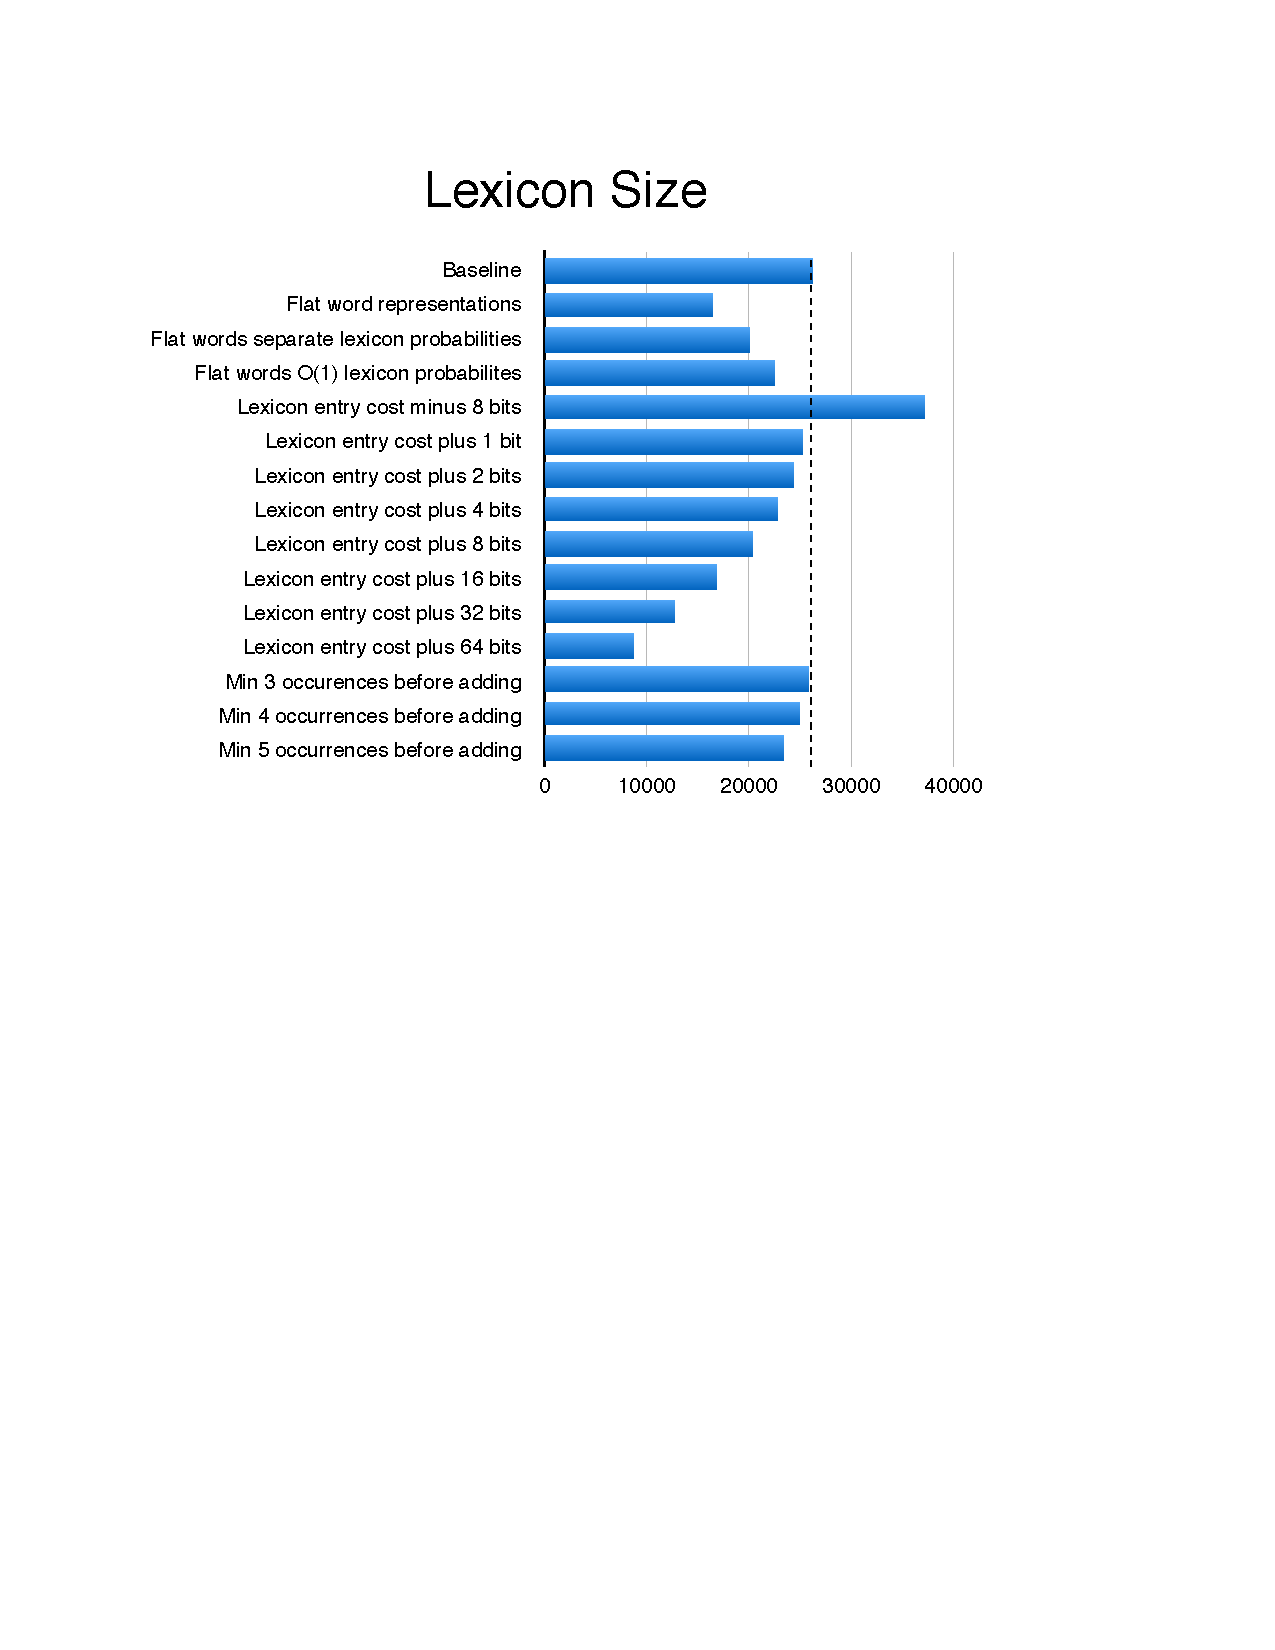
\includegraphics{./figure/lexicon_size.pdf}
  \end{figure}

  \begin{figure}[h]
  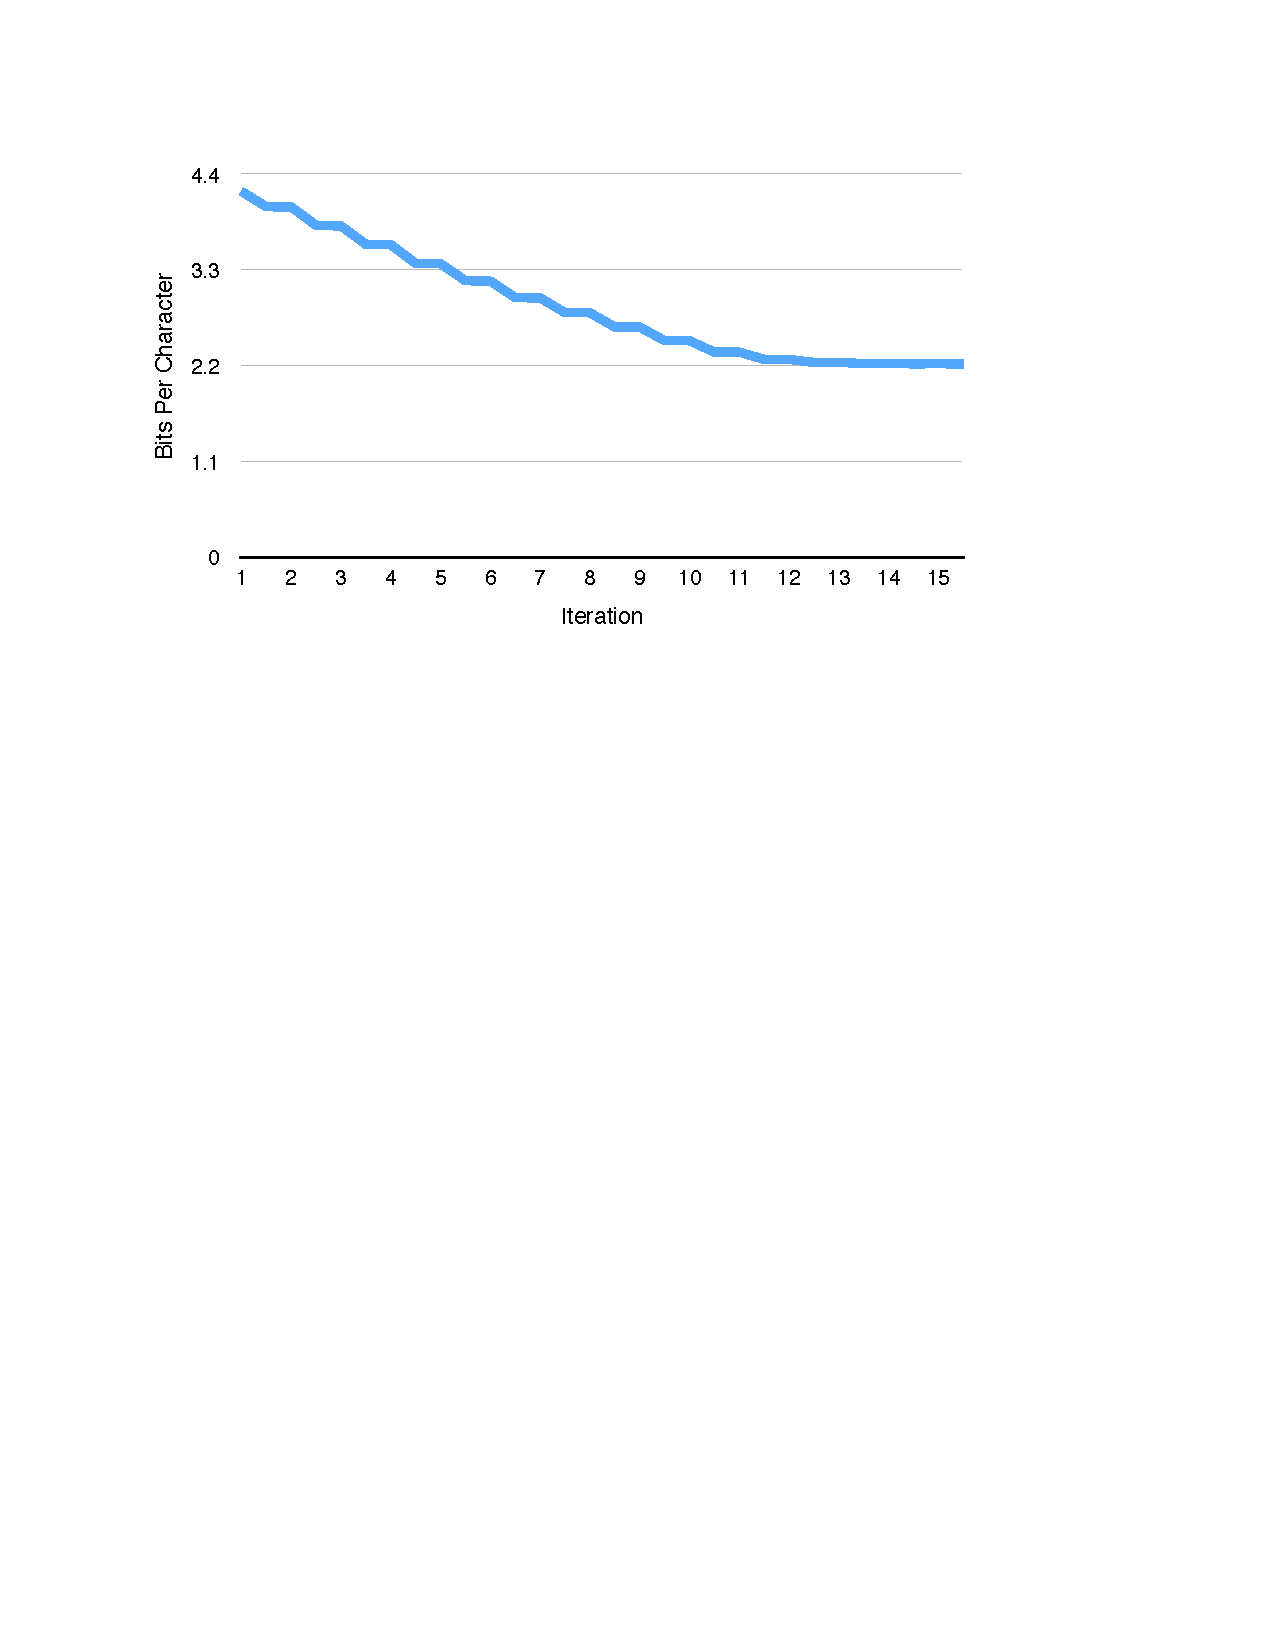
\includegraphics{./figure/bit_of_char_per_iteration.pdf}
  \end{figure}

  \begin{figure}[h]
  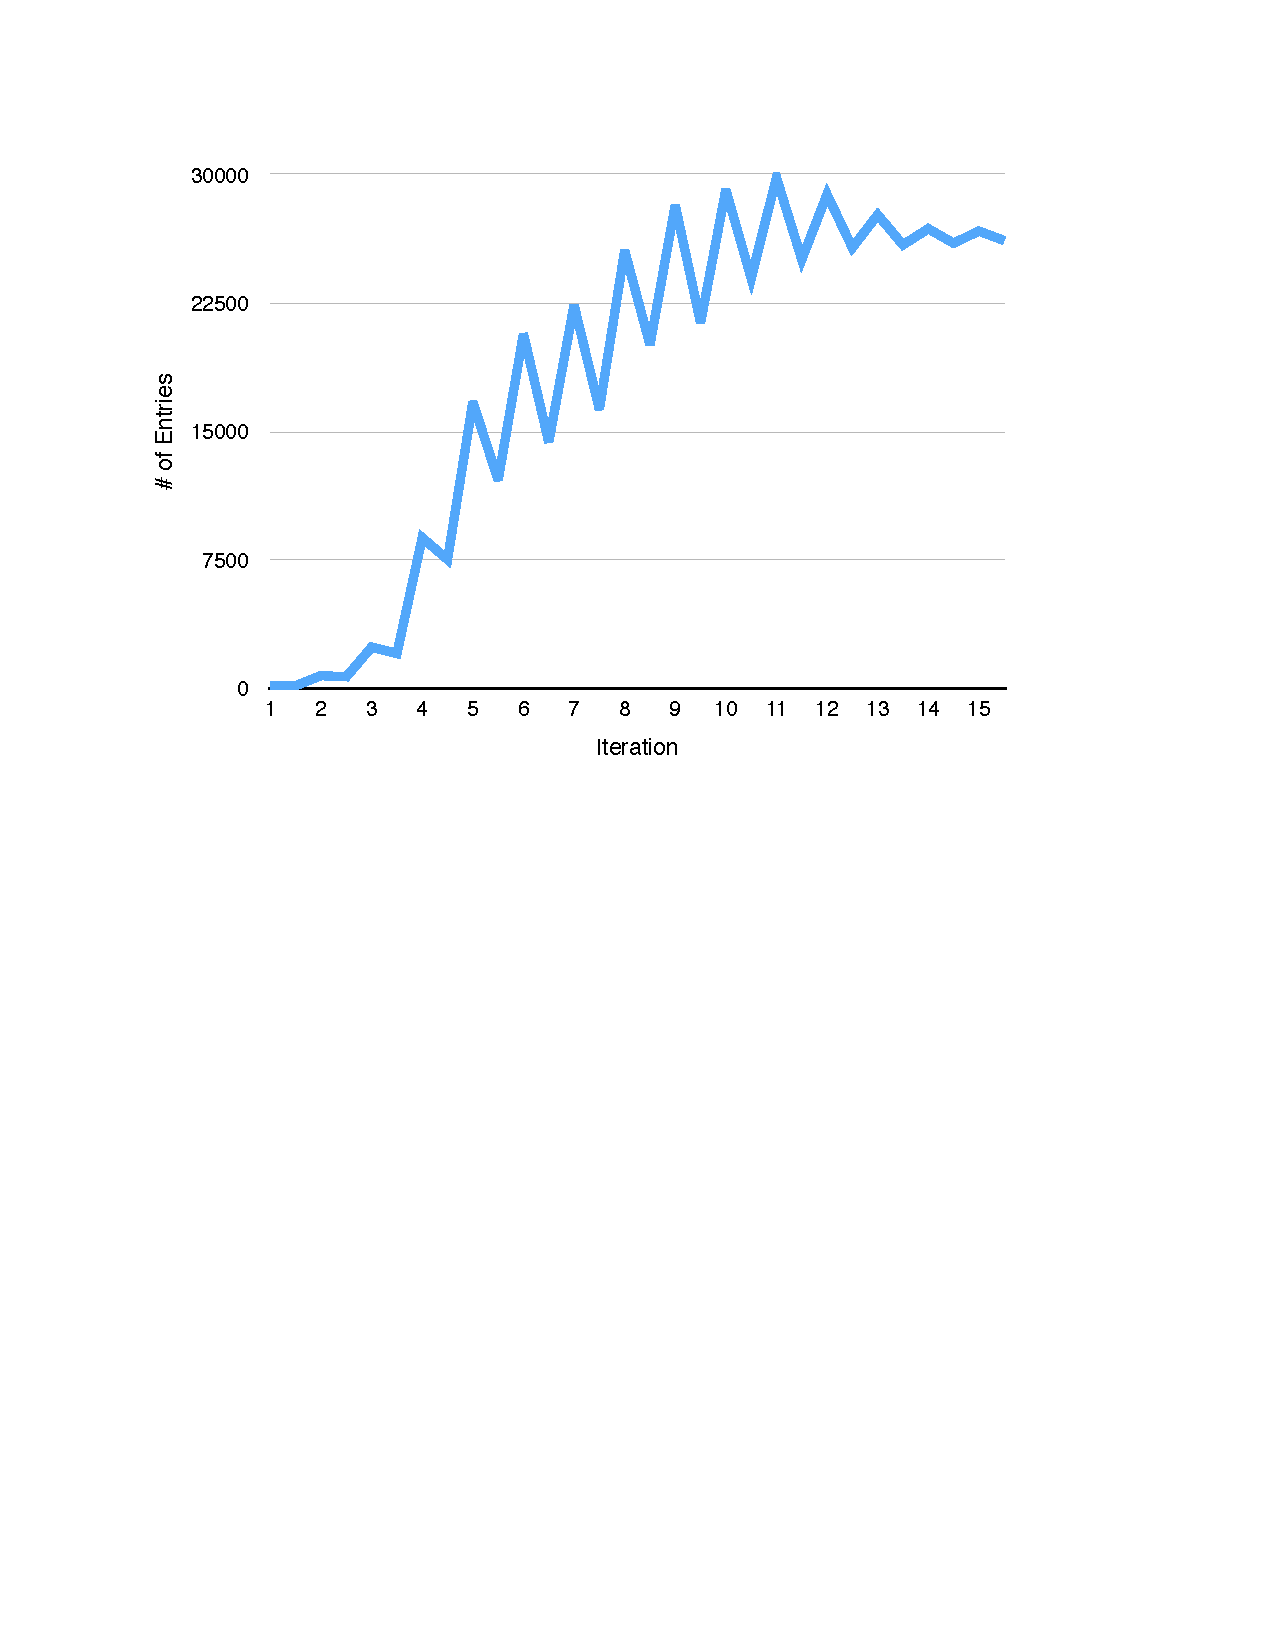
\includegraphics{./figure/entropy_per_iteration.pdf}
  \end{figure}

  During our baseline running, 60\% of found word are exactly correct, 40\% are incorrect. We investigate these incorrect found words deep, and try to categorize what kind error types they belong to. As you can see below, about 43\% of those words combines two true word together as one segmented word, 18\% is our tool find this word but doesn't split it at correct ending character, the error about finding this word but not splitting it at correct starting character also takes almost 18\%. 8.7\% is caused by combining three real words together as one word, while 1.6\% comes from quad+ words combination. We also notice that 6.2\% is for a true word, our tool splits it into several fragements. Sometimes, our tool would find a word, but adding suffix and prefix from its neighbor words, taking 3.3\%.

  \begin{figure}[h]
  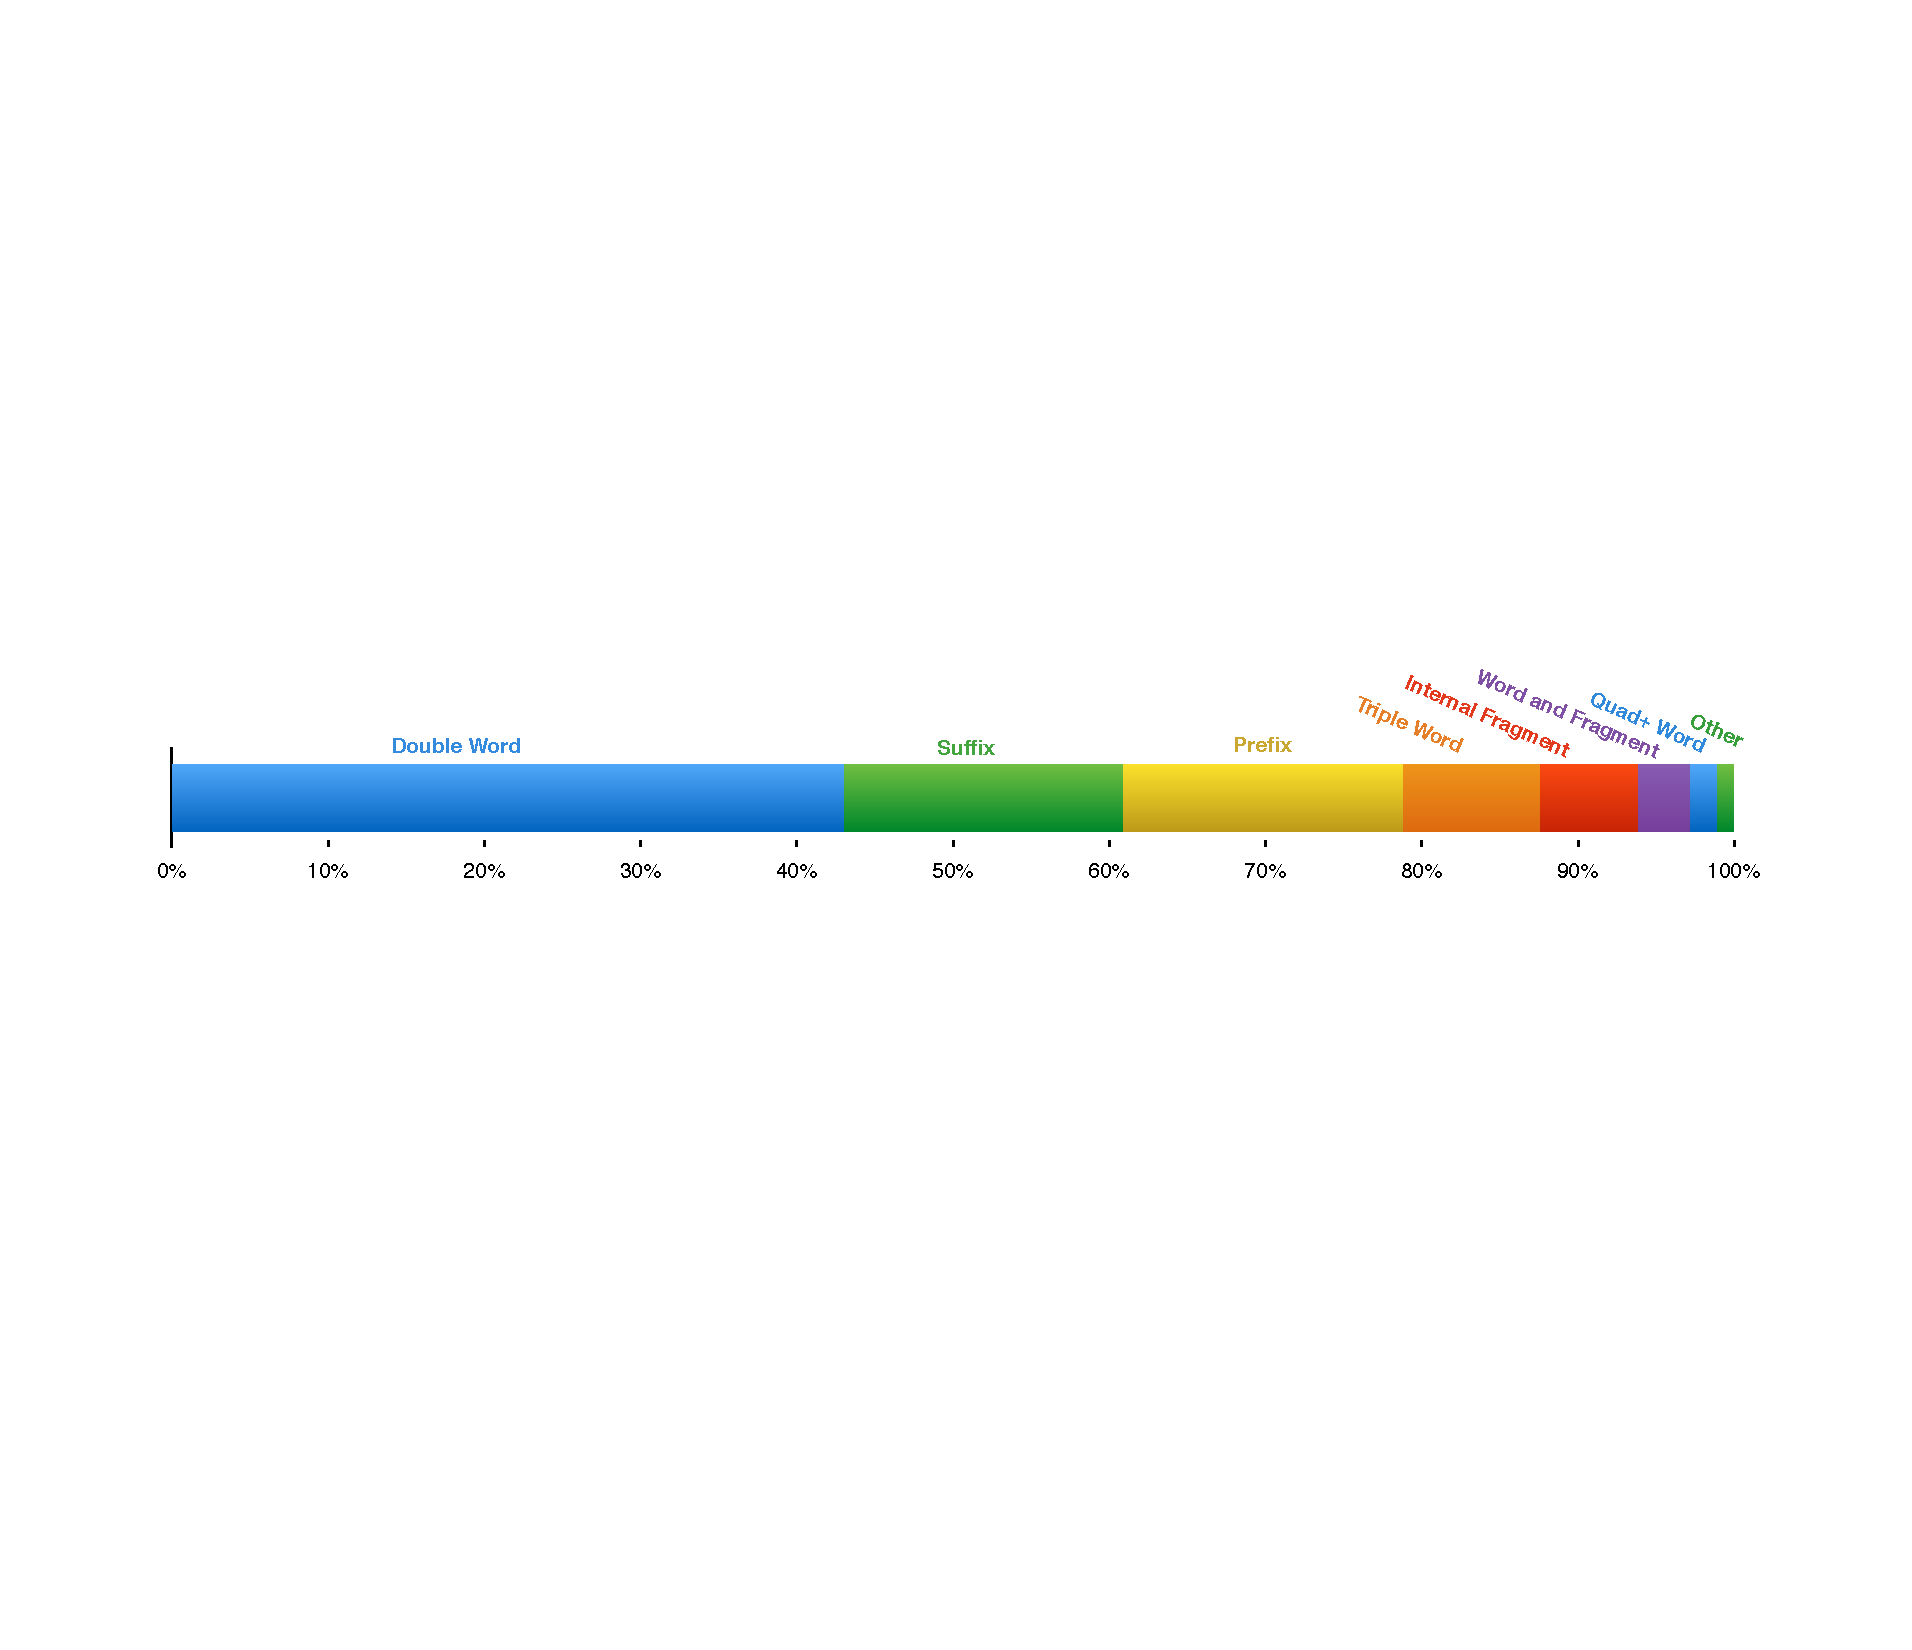
\includegraphics[scale=0.6]{./figure/error_nature_classfier.pdf}
  \end{figure}
  
  \begin{figure}[h]
  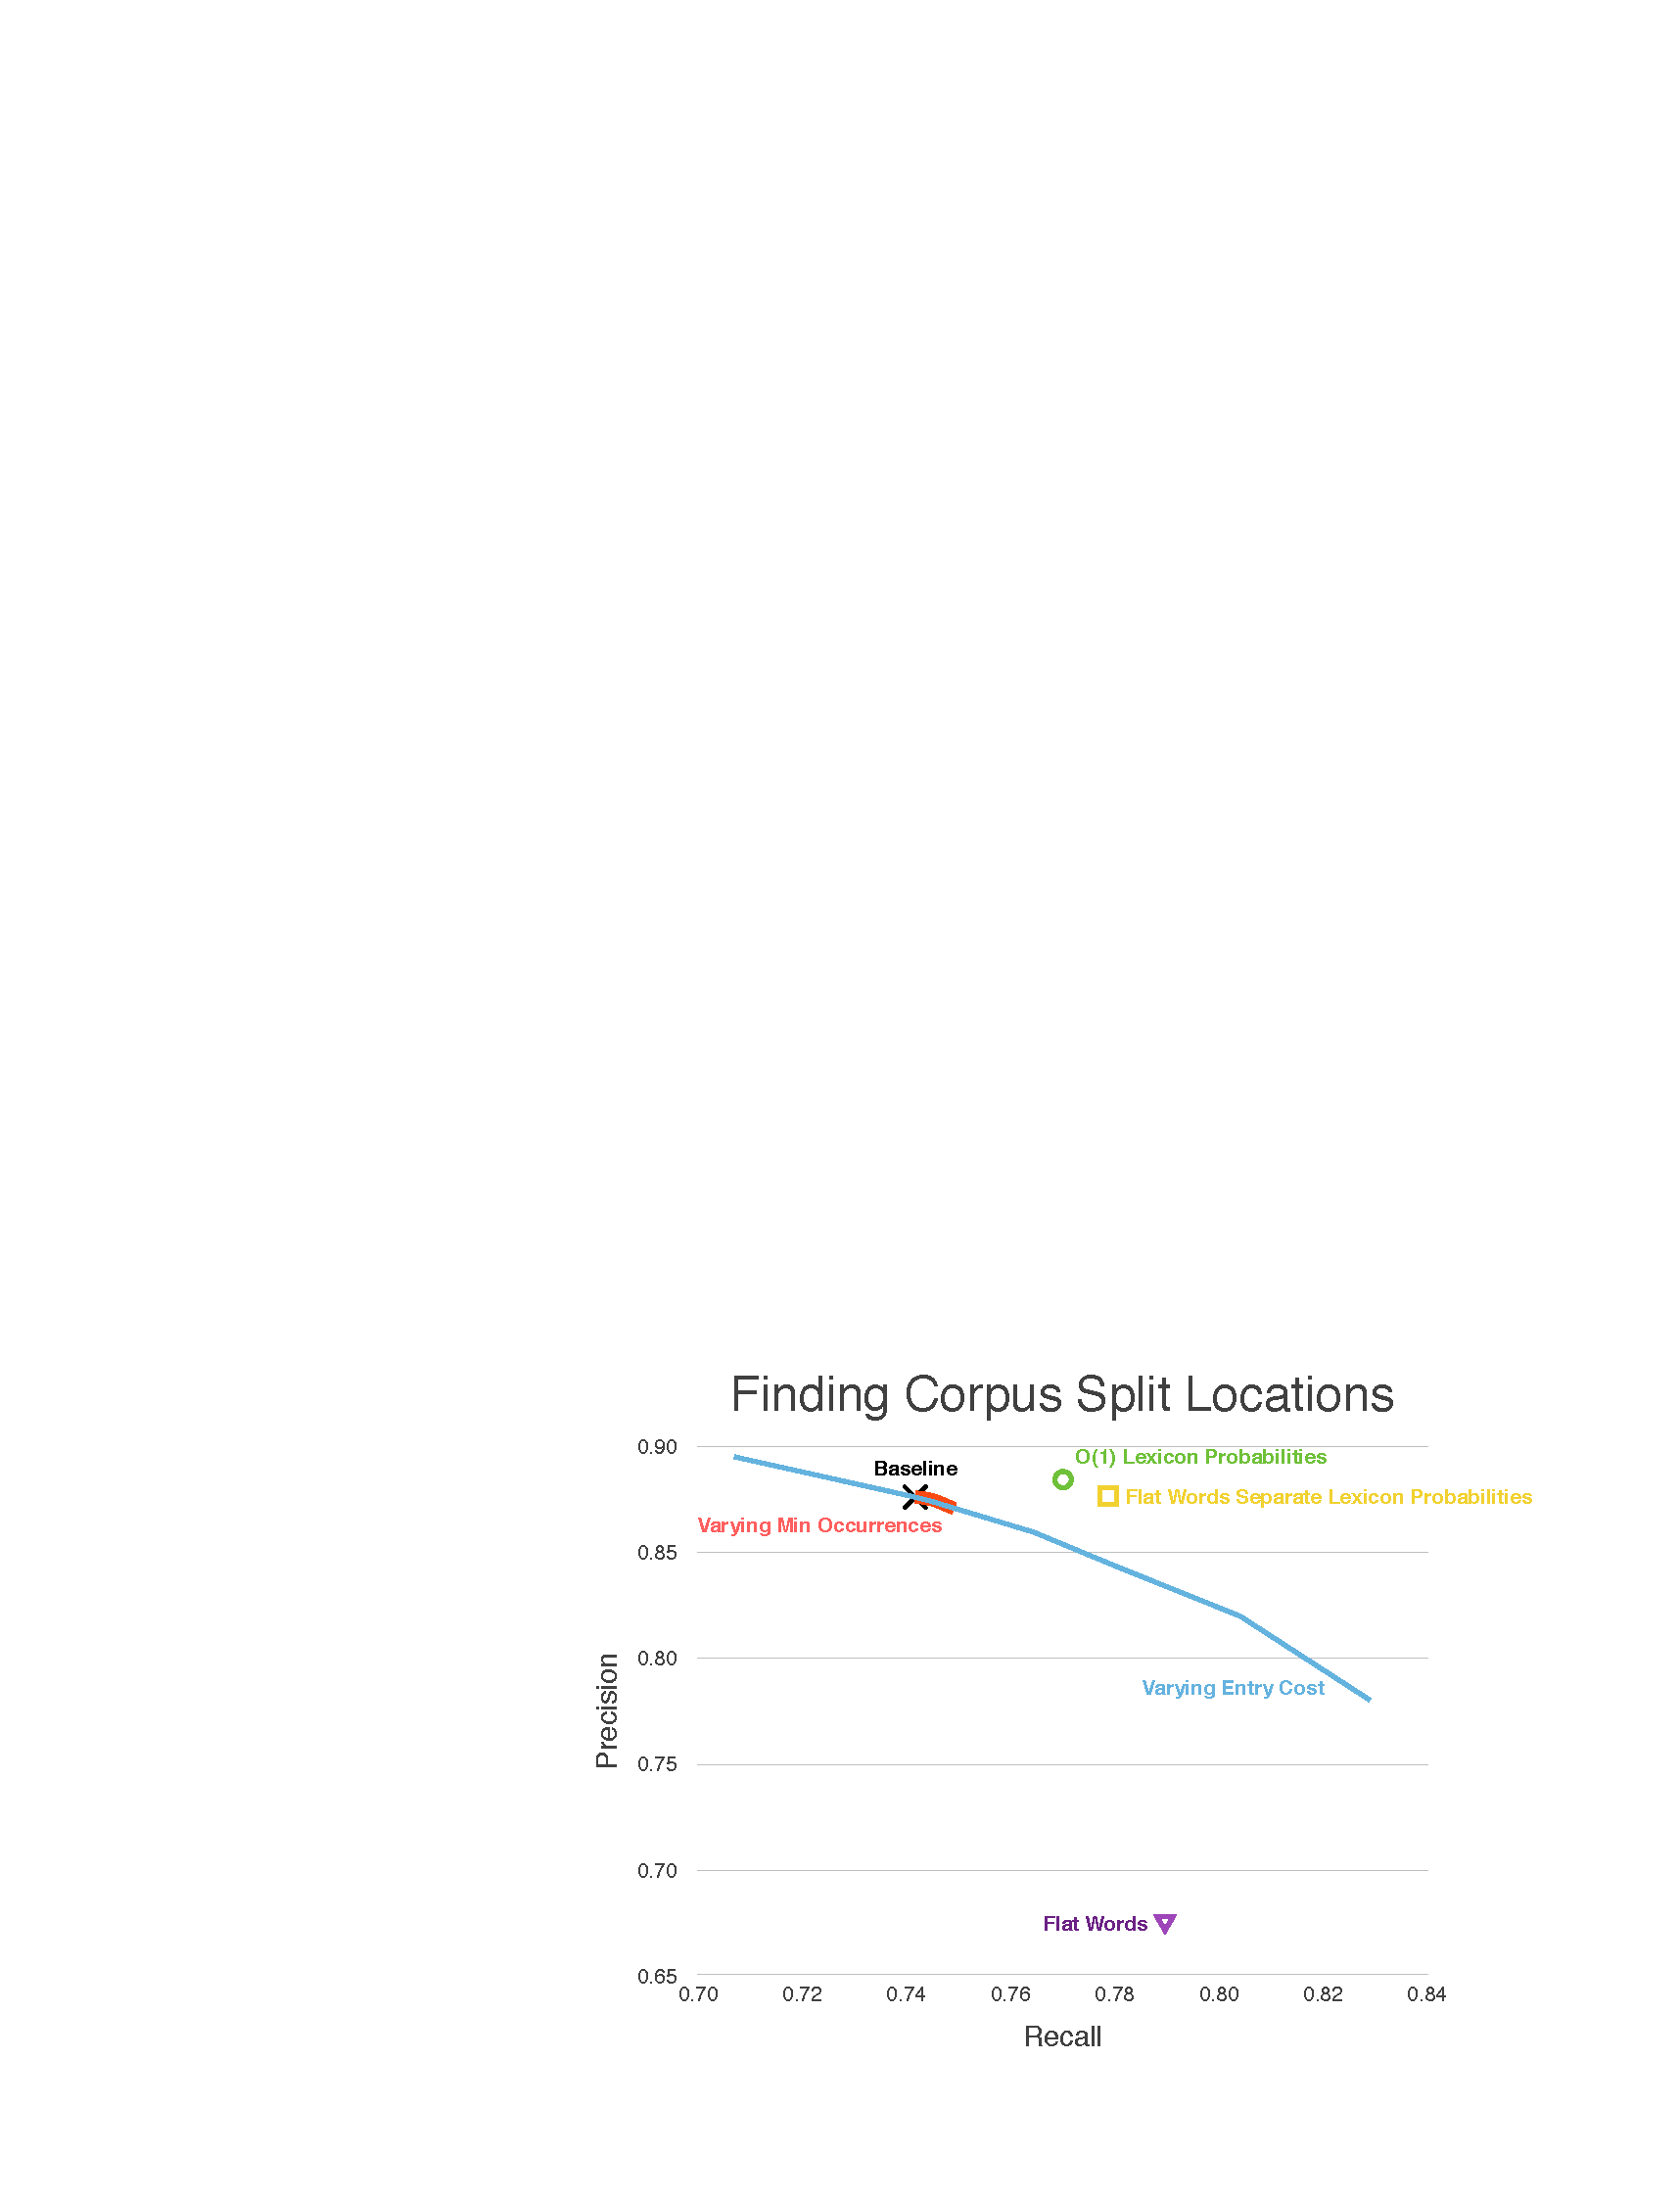
\includegraphics{./figure/finding_corpus_split_location.pdf}
  \end{figure}

  \begin{figure}[h]
  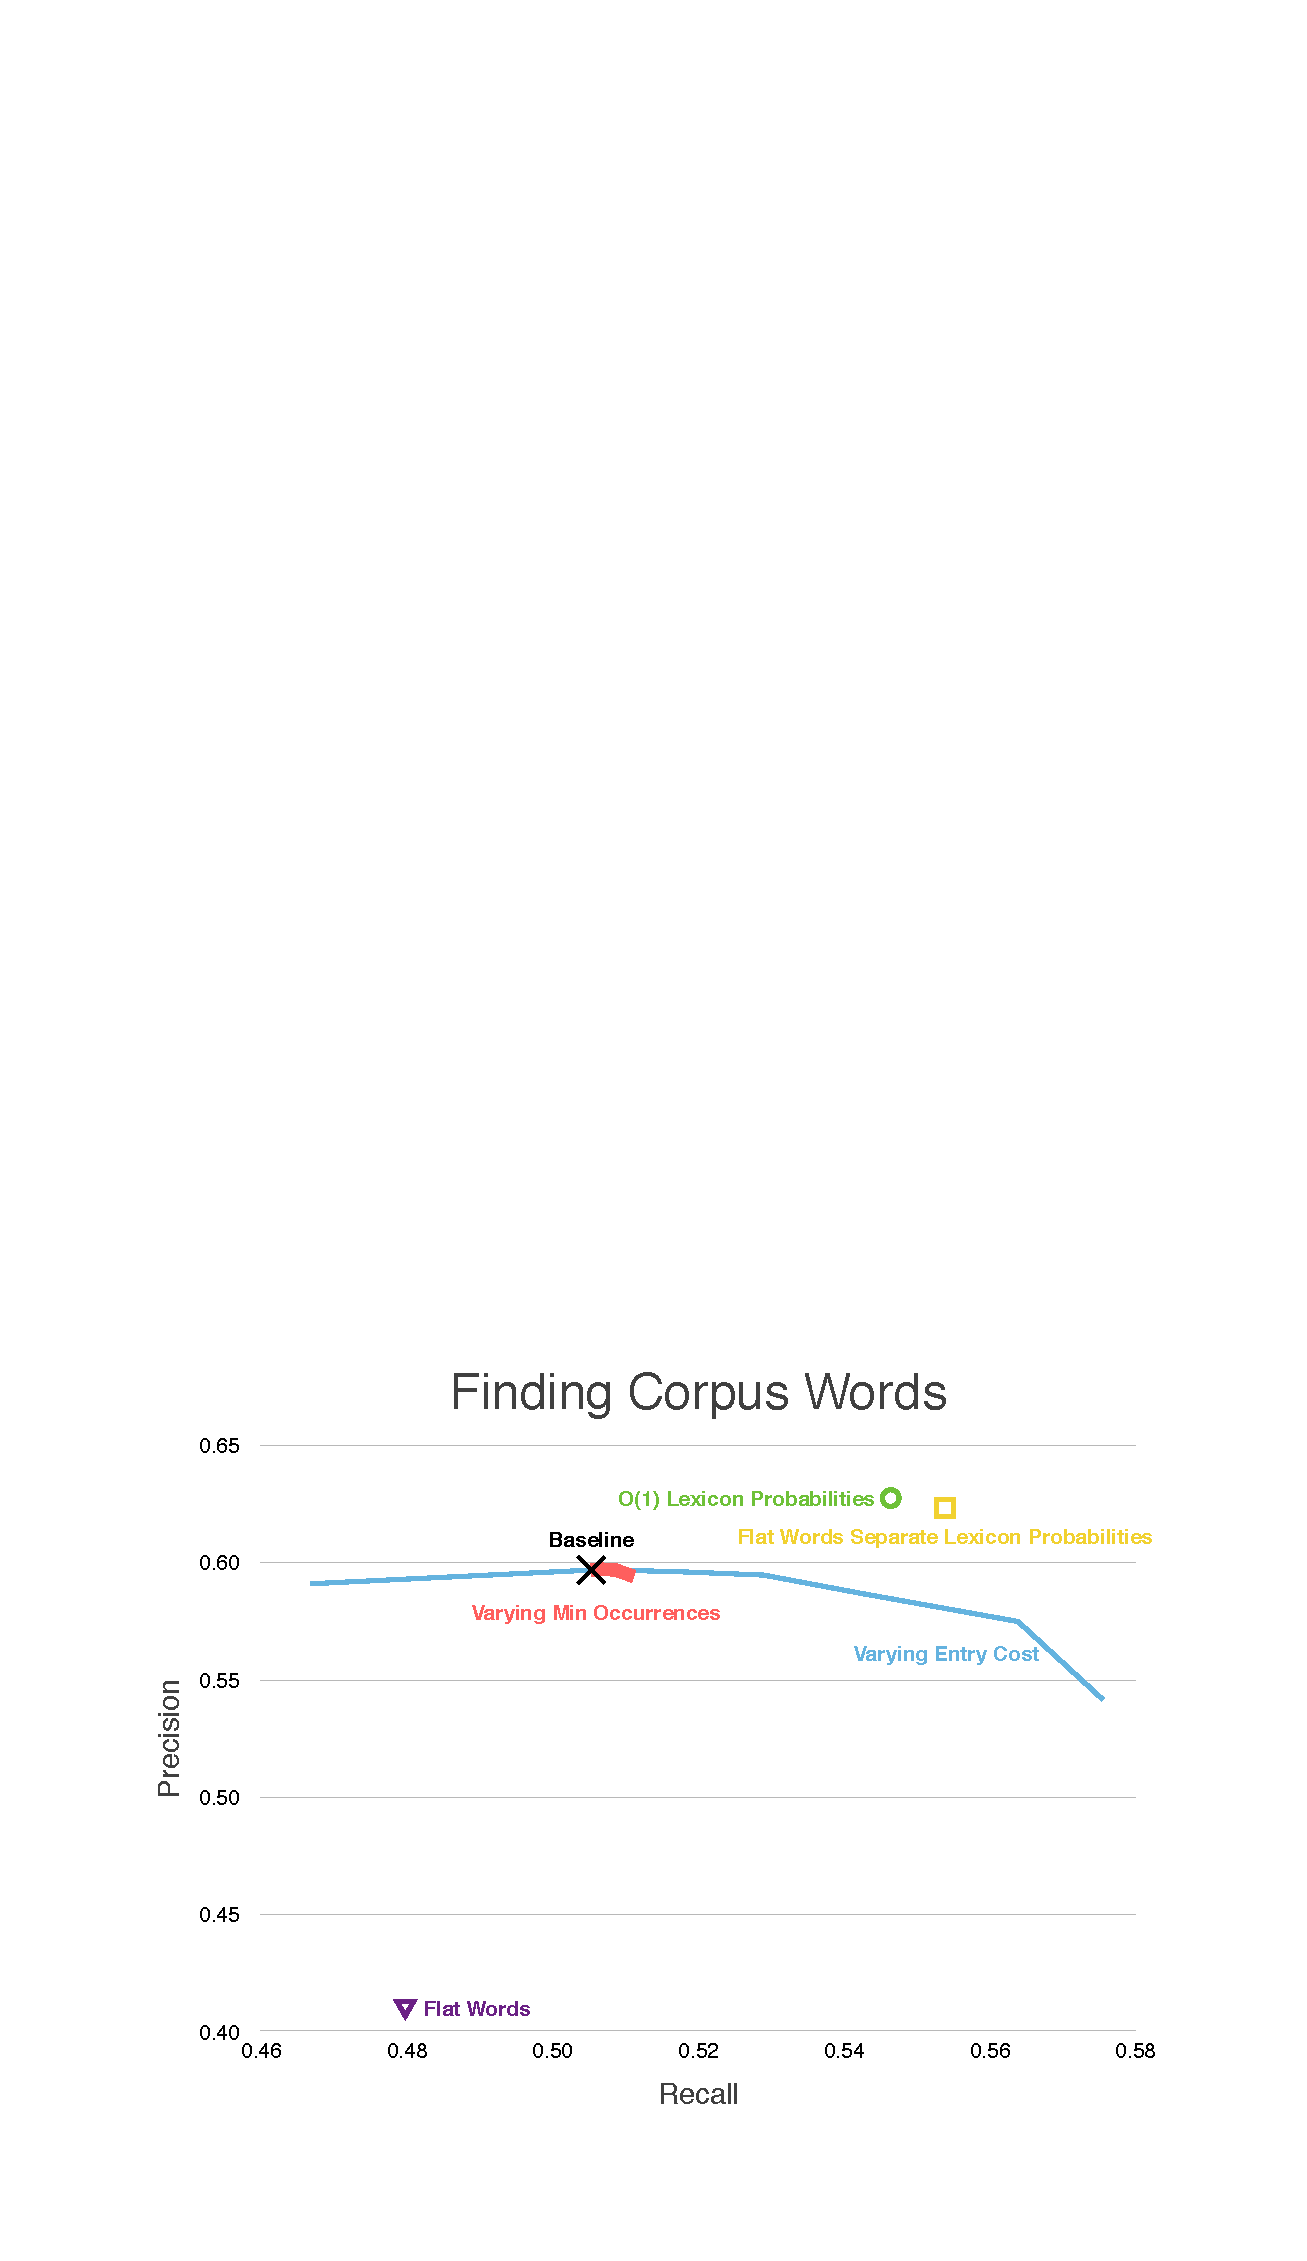
\includegraphics{./figure/finding_corpus_word.pdf}
  \end{figure}

  \section*{Discussion}

  what do the results mean

  \section*{Ideas for Improvement}

  ideas for improvement

\end{document}
